This project consists on the implementation of the paper \cite{CAPO201756}, which was developed by Marco Capó and Aritz Pérez and Jose A. Lozano in the Knowledge-Based Systems journal. The paper aims to approximate the performance of KMeans, one of the most widely used clustering methods for massive datasets, while reducing the number of distance computations required to achieve a good clustering solution. The solution proposed by the authors is based on the recursive partition of the dataset following an heuristic that they call Recursive Partition based K-Means. 

\section{Definitions}

In their paper, the authors start by defining mathematically a partition, subset and the cardinality of the subset and the center of mass. They define a partition $P$ as a collection of disjoint subsets $S$ which the union of them results in the whole dataset $D$. They define the weight of the subset as the cardinality of it $|S|$ and the center of mass as the mean of all the points in the subset $\bar{S} = \frac{\sum_{x \in S} x }{|S|}$.

\section{Proposed solution}
The solution proposed by the authors uses partitions as the units for fitting weighted Lloyd algorithms instead of using the data points from the dataset. The dataset is split into subsets each of them is represented by a representative sample and the cardinality of the subset.

The authors propose to divide the space where the dataset lies and partition it recursively using a quadtree, where the entire space of the subset is divided into $2^d$ subspaces. In a $2D$ space, the plane would be divided into quadrants, then each of the quadrants would be divided into 4 "subquadrants" and so on. Thanks to kthis heuristic, the number of elements is controlled, always satisfying $|P|<n$ or in other words, that the length of the partition ant every given moment is smaller than the number of instances in the dataset.

In \ref{fig:partitions} we show a $2D$ gaussian mixture with 3 gaussian and an overlap of 5\%. Each partition has the subsets in different colors to be able to discriminate them easily. Each partition contains subsets thinner than the previous one, and the subsets of the partition $P_{i+1}$ are generated by spliiting subsets from the partition $P_i$. The authors define that a partition $P_i$ is thinner than $P_j$ if every subset of $P_i$ can be written as the union of subsets of $P_j$ which applies in the case of the RPKM algorithm.

\begin{figure}[!ht]
    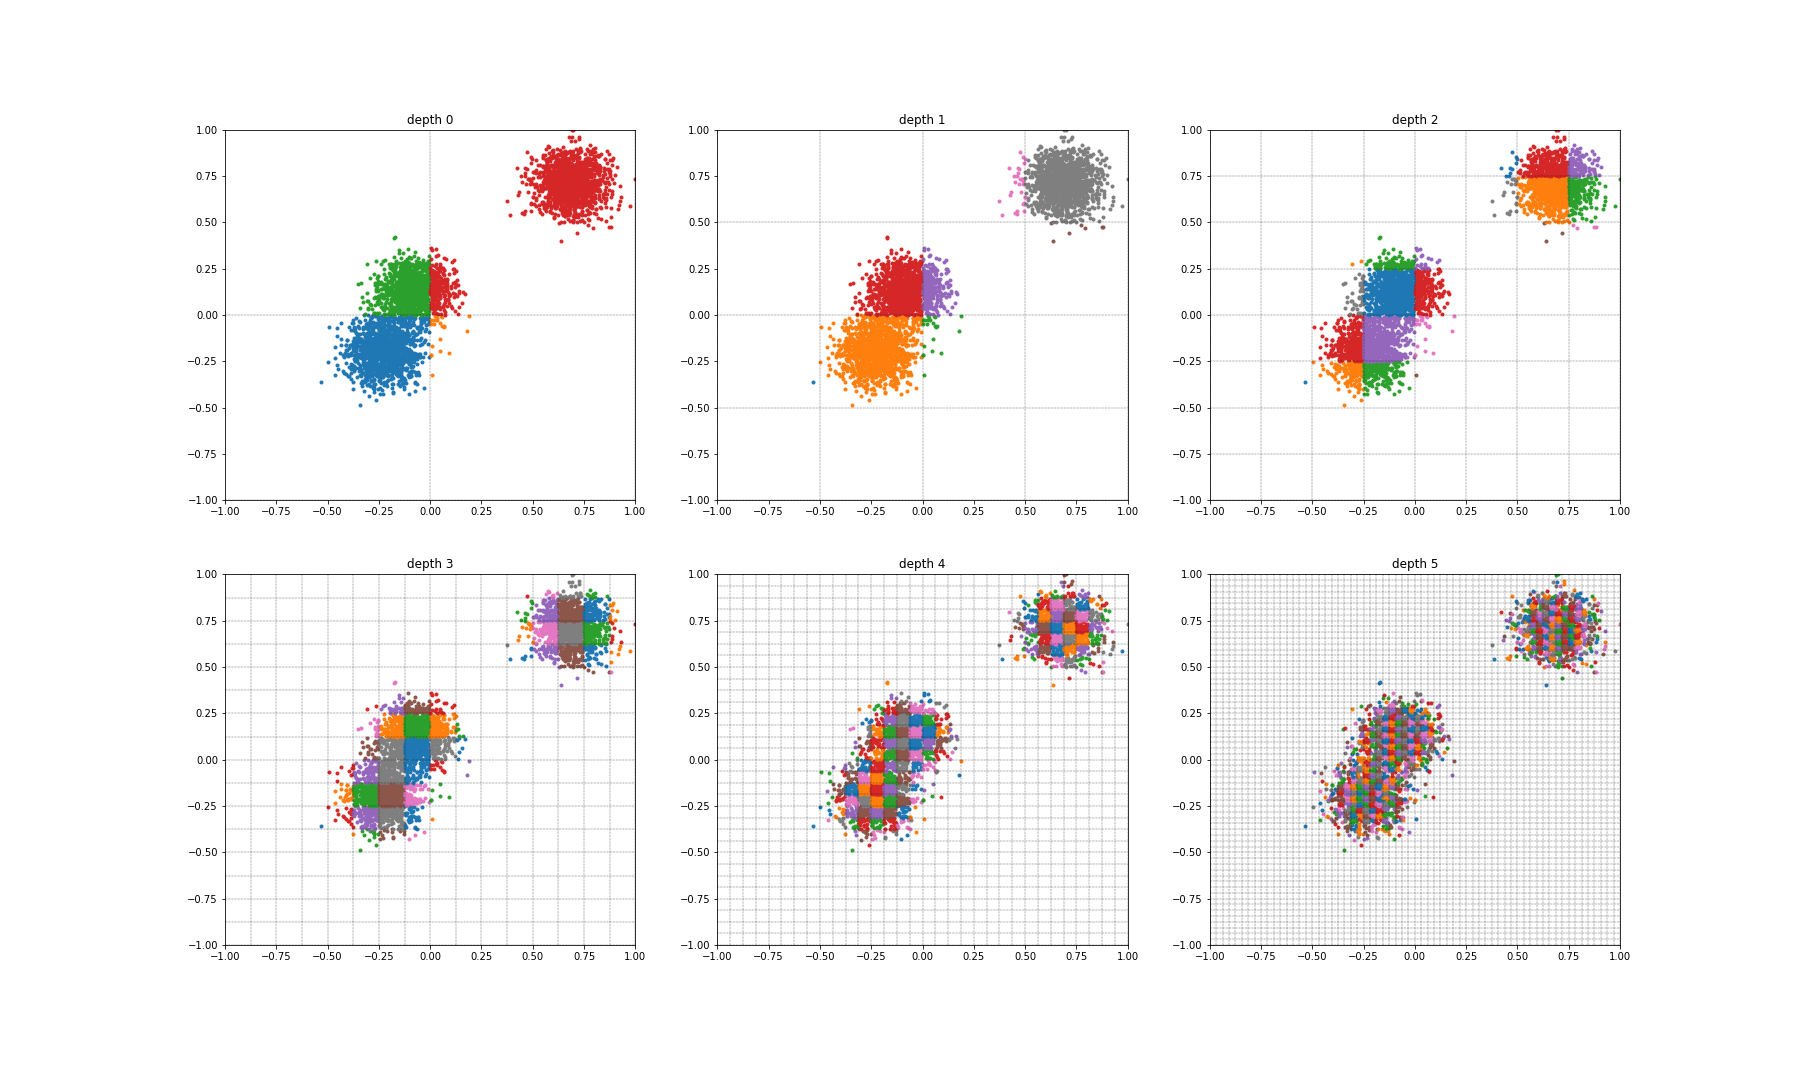
\includegraphics[width=\linewidth]{images/alldepths.png}
    \caption{Partition example for a 2d gaussian mixture}
    \label{fig:partitions}
\end{figure}

The authors propose an approach where for each one of the partitions mentioned above, a weighted Lloyd (WL) algorithm is trained and the centers extracted in each of the iterations is used as initialization for the next partition. This drastically reduces the number of distance computations that the algorithm realizes as the number of representative samples that will be used to fit the WL algorithm is always smaller than $n$. 

\begin{algorithm}[H]
    \SetAlgoLined
    \KwIn{Set of representatives $\{\bar{S}\}_{S \in P}$ and weights $\{|S|\}_{S \in P}$, for the partition $P$. Number of clusters K and initial set of centroids $C_0$.}
    \KwOut{Set of centroids $C_r$ and the Corresponding clustering pattern $G_r$}
    $G_0 \leftarrow C_0; r=0$\;
    \While{not Stopping Condition}{
        $r = r+1$\;
        $C_r \leftarrow G_{r-1}$\;
        $G_r \leftarrow C_r$\;
    }
    \KwRet{$C_r$ and $G_r$}
    \label{algo:wl}
    \caption{WL algorithm}
\end{algorithm}

The weighted Lloyd algorithm is shown in \ref{algo:wl} and it shows that given a set of representatives, a set of weights, a number of clusters and an initial set of centroids $C_0$, it iteratively improves the centers by assigining the weighted mean of all the instances in a group or cluster as their centroid and then computing the group of each instance as the center index that is closer to each instance.

\begin{algorithm}[H]
    \SetAlgoLined
    \KwIn{Dataset D, number of clusters K, maximum number of iterations m}
    \KwOut{Set of centroids approximation $C_i$}
    Compute the set of weights and representatives of the sequence of thinner partitions, $P_1, \dots ,P_m$, backwards. \;
    i := 1\;
    \While{not Stopping Criterion}{
        Update the centroid's set approximation, $C_i = \{c_j^i\}_{j=1}^K$: $C_i = WL(\{\bar{S}\}_{S \in P_i}, \{|S|\}_{S \in P_i}, K, C_{i-1})$\;
        $i = i+1$
    }
    \KwRet{$C_i$}
    \label{algo:rpkm}
    \caption{RPKM algorithm}
\end{algorithm}

The RPKM algorithm is exposed in \ref{algo:rpkm}. In the algorithm we can appreciate that the autors compute all the weights and representatives for the given dataset D and then iteratively update the centers for each iteration by performing a WL computation on the representative samples and cardinality of the subsets. Additionally, they use the cluster centers from the previous RPKM iteration as initialization.

Both algorithms hav similar stop criteria, a threshold on the distance between the centers of the previous and new iteration and a maximum number of iterations. However, the authours have removed the distance limitation in their implementation in order to see the effects of the algorithm fully.
